%!TEX root = ../07-Electrical-Components.tex
\chapter{Temperature Dependence of Electrical Resistance}

\begin{figure}[tbp]
	\centering
	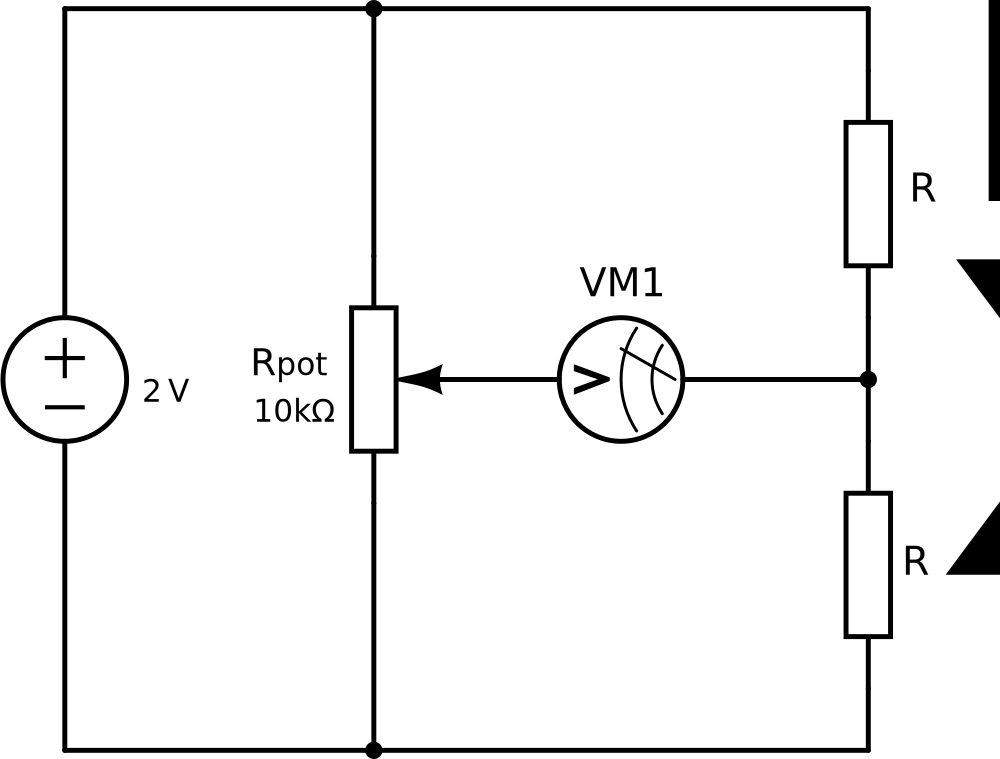
\includegraphics[width=.4\textwidth]{img/sch-wheatstone.pdf}
	\caption{Wheatstone Bridge Schematic}
	\label{sch:wheatstone}
\end{figure}

\def\tcsubfigwidth{0.6\textwidth}
\def\tcgraphicswidth{1.1\textwidth}

\begin{figure}[tbp]
	\centering
	\begin{subfigure}{\tcsubfigwidth}
		\centering
		\includegraphics[width=\tcgraphicswidth]{data/plots/tempco-ntc.pdf}
		\caption{NTC}
		\label{plot:tempco:ntc}
	\end{subfigure}
	\begin{subfigure}{\tcsubfigwidth}
		\centering
		\includegraphics[width=\tcgraphicswidth]{data/plots/tempco-pt100.pdf}
		\caption{PT100}
		\label{plot:tempco:pt100}
	\end{subfigure}
	\caption{Temperature Dependence of NTC and PT100 resistance}
	\label{plot:tempco}
\end{figure}

The temperature dependence of the resistances of an NTC and a PT100 thermal sensor are examined.

\section{Setup}

Temperature is controlled with an oven and is ramped from ambient temperature to \SI{200}{\celsius}.
A K-type thermocouple is used to monitor the current temperature.

The resistance of the device under test is measured with a Wheatstone bridge (\autoref{sch:wheatstone}).
A Wheatstone bridge allows two resistances to be compared precisely, the overall accuracy is unaffected by the load and characteristics of the current- or voltmeter, thus is only limited by the tolerances of the used resistors.
The voltage differential across the middle of the bridge is measured with a digital multimeter.
A multiturn potentiometer fitted with a turn-counting dial is used to set and read the resistance ratio on the left side of the bridge.

The resistance $R_\text{x}$ of the DUT is calculated as
\begin{equation}
	\frac{R_\text{set}}{R_\text{pot}} = \frac{R_\text{x}}{R_\text{x} + R_\text{ref}}
	\quad \implies \quad R_\text{x} = R_\text{ref} \; \frac{R_\text{set}}{R_\text{pot} - R_\text{set}},
\end{equation}
with the resistance of the potentiometer $R_\text{pot}$, it's lower arm $R_\text{set}$ and the reference resistor $R_\text{ref}$.

The measured value is most accurate when $R_\text{x}$ and $R_\text{ref}$ are roughly equal, so the reference resistor is changed multiple times throughout the measurement series.

\section{Evaluation}

A graph of the measured values is shown in \autoref{plot:tempco}.

The theoretical resistance function for each component is fitted to the data (uncertainties are purely statistical):

\textbf{NTC:}
\begin{gather*}
	R(T) = a \cdot \mathrm{e}^{\frac{b}{T}} \tag*{(T in \si{\kelvin})}\\
	a = \SI{2.50(4)e-2}{\ohm}	\qquad	b = \SI{3628(6)}{\kelvin}
\end{gather*}
\textbf{PT100:}
\begin{gather*}
	R(T) = R_0 \cdot \left(1 + \alpha \, T \right) \tag*{(T in \si{\celsius})}\\
	R_0 = \SI{104.1(8)}{\ohm}	\qquad	\alpha = \SI{3.64(8)e-3}{\kelvin^{-1}}
\end{gather*}

The statistic uncertainty of the NTC fit parameters is very low, though comparing them to results of different groups, they each differ by more than \SI{30}{\percent}.\\
The fit parameters for the PT100 are close to the nominal values of $R_{0,\text{lit}} = \SI{100}{\ohm}$ and $\alpha_\text{lit} = \SI{3.85e-3}{\kelvin^{-1}}$.
The nominal values are not within range of the estimated statistical tolerances, however they are covered by the linearity (\SI{1.5}{\percent}) and absolute accuracy (\SI{3}{\percent}) of the potentiometer.

The NTCs unusual property of conducting better at higher temperature makes it suitable as a passive inrush current limiter.
When used as an inrush current limiter, it's resistance is initially high, then drops off as it heats up from the current passing through it.
This is highly important when connecting capacitive loads to low-impedance power supplies such as mains voltage.\\
NTCs can also be used as fluid level meters.
In this application a current is passed through it, making it both a heating element and a temperature sensor.
When it is submerged in fluid it can't heat up, so its resistance is high.
If the fluid level drops below the NTC, it will heat up, lowering its resistance.
This has the effect of increasing the total heating power (as long as the NTCs resistance is smaller than the power supply's impedance), generating positive feedback.\\
NTCs are also used as plain temperature sensors, though the low initial accuracy must be compensated by calibrating devices individually unlike PT100 elements, which are manufactured to specific tolerances.
